\section{Our Approach}
\label{sec:approach}

Neural network-based dependency parsing approaches in natural language processing (NLP)~\cite{chen-manning-2014-fast} project words in a sentence into an embedding space to successfully learn the semantic relationships between them. Thus, we sought motivation for \tool's design, geared towards learning the control-flow and program dependencies between statements in programs. Moreover, the quality of the statement embeddings determines how accurately our tool can predict the program dependence relations. Thus, enhancing them by incorporating context from both within and across the statements is crucial. For example, the knowledge of the declaration of a variable in one statement and its reference in another helps identify the \textit{def-use} chain between them. Also, it is important to model the effect that a statement has on the other statements. For example, such information helps identify the scope of a given statement. Finally, we model our problem as a pairwise dependence decoding task, wherein the combination of all predicted edges across the statement pairs in a program can be formalized as a directed graph, i.e., its CFG/PDG.

\subsection{Model Architecture}
\label{sec:arch}

\begin{figure*}[ht]
\begin{center}
    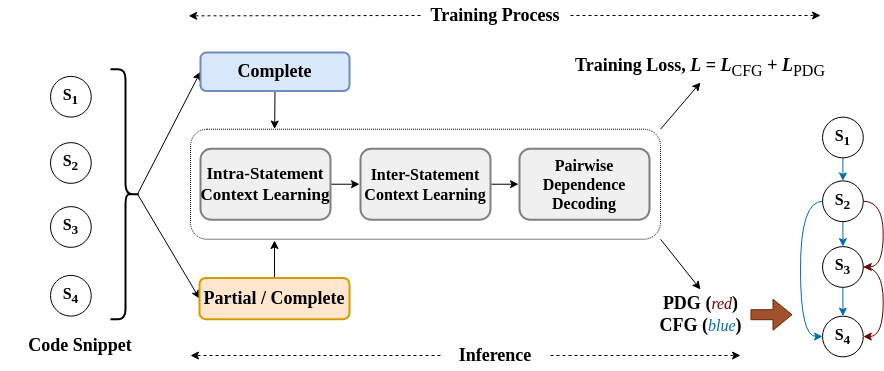
\includegraphics[width=0.8\textwidth]{icse23-demo-figures/demo-arch.png}
    \caption{\tool training and inference pipeline to enable dependence analysis for both partial and complete code.}
    \label{fig:model}
    \vspace{-10pt}
\end{center}
\end{figure*}
In Figure~\ref{fig:model}, we present the general model architecture of \tool. We incorporate various context-learning modules to capture the well-defined structure and semantics in source code. In this section, we describe each of these components.

\subsubsection{Contextualization}
Effective contextualization is a key idea driving \tool's design. We enable this via a hierarchical, self-attention network (SAN)-based architecture, where each sub-network is intended to capture different aspects of contextualization. Its details are as follows:

\begin{itemize}[leftmargin=*, listparindent=\parindent, parsep=0pt, itemsep=\topsep]
%\begin{itemize}[listparindent=\parindent, parsep=0pt, itemsep=\topsep]
    \item \underline{\textit{Intra-Statement Context Learning (IntraS-CL)}}. To relay the syntactic and semantic knowledge of code tokens within individual statements globally, intra-statement contextualization is crucial. We enable this via a \textit{1-Layer} (i.e., $N_X$$=$$1$) Self Attention Network (1L-SAN). The self-attention layer in an 1L-SAN inputs $x_1, x_2, ..., x_n \in \mathbb{R}^d$, performs self-attention once by projecting the inputs from all attention heads $\in\mathbb{R}^{d_h}$ into the head dimension space $d_h$ via linear transformations, and generate outputs $y_1, y_2, ..., y_n \in\mathbb{R}^d$ which are linear combinations of the concatenated attention head values. We use one attention head (i.e., $h$$=$$1$) for the self-attention layer in 1L-SAN, and the size of the input representations, i.e., $d$ is set to 512.

    \hangindent=0.7cm For a program comprising $N$ statements $s_1, s_2, ..., s_N$, \tool takes as input a concatenation of $N$ sequences of $M$ tokens each, $\langle t_1^{(1)}$, $t_2^{(1)}$.., $t_M^{(1)} \rangle$, ..., $\langle t_1^{(N)}$, $t_2^{(N)}$.., $t_M^{(N)} \rangle$. Next, each token sequence $\langle t_1^{(i)}$, $t_2^{(i)}$.., $t_M^{(i)} \rangle$ is input to the 1L-SAN for intra-statement contextualization. Previous works~\cite{radford2019language, liu2019roberta} have demonstrated the advantages of a byte-level Byte-Pair Encoding (BPE)-scheme for tokenization. We follow suit to train a byte-level BPE tokenizer for converting a given statement into a sequence of tokens. Here, $M$ is the maximum number of tokens allowed in a statement. For statements with token sequences having ${<}M$ tokens, a special \textit{[PAD]} token is appended. In contrast, token sequences having ${>}M$ tokens are truncated to $M$ tokens.

    \item \underline{\textit{Inter-Statement Context Learning (InterS-CL)}}. The knowledge of the surrounding statements in the context of a given statement helps \tool model the dependencies between them better. We enable this via a multi-layer bidirectional Transformer encoder based on the work by Vaswani {\em et al.}~\cite{Vaswani-2017}. Owing to its common usage, we will omit exhaustive background details on Transformers' model architecture and will refer the readers to ~\cite{Vaswani-2017}. We set the number of layers in the Transformer encoder, i.e., $N_Y$ to 6. We employ 4 attention heads, i.e., $h$$=$$4$ to increase parallelization (since $d_h$$=$$\frac{d}{h}$, i.e., $d_h$$=$$128$) and learn different aspects of the syntactic and semantic structure in the statements, while still being interpretable. We also set the feed-forward module size to be 4 times that of the size of the input representations $d$, i.e., 2048. Overall, Transformer in InterS-CL phase inputs local context-aware statement representations $u_i \in \mathbb{R}^d$ for all statements $s_i$ in a given program, and outputs statement representations $v_i \in \mathbb{R}^d$ that are both local and global context-aware.
\end{itemize}

\subsubsection{Pairwise Dependence Decoding}
From the sequence of contextualized statement representations $v_i \in\mathbb{R}^d$ corresponding to all the statements $s_i$ in a program, pairs such as $\langle v_x, v_y \rangle$ (1$\leq x, y\leq$ N) are taken to detect the presence of CFG/PDG edges between two statements $s_x$ and $s_y$. We leverage 2-layered multi-layer perceptron networks (each for detecting the CFG and PDG edges, i.e., MLP\textsubscript{CFG} and MLP\textsubscript{PDG}, respectively) in this phase, which are scored as per the following equation:
\begin{equation}
\centering
    score\textsubscript{rel}(x, y) = MLP\textsubscript{rel}(v_x \circ v_y \circ (v_x * v_y) \circ |v_x - v_y|) \nonumber
\end{equation}
where $\circ$, $*$ and $|.|$ correspond to concatenation, element-wise
product, and absolute element-wise difference operations respectively;
and \textit{rel} represents either the control-flow or program
dependence relations. 
%and \textit{rel} $\in$ \{CFG, PDG\}. 
Attaining a $score\textsubscript{rel}(x, y) >
0.5$ represents the detection of the corresponding CFG/PDG edge from
statement $s_x$ to statement $s_y$. The combination of all the CFG/PDG
edges extracted via such an arc-factored approach is realized as the
CFG/PDG for the given program.

\subsection{\bf Training Process}
Training \tool requires the knowledge of whether a CFG or PDG edge occurs between any two statements in the program. This is due to its design as an inter-statement dependence prediction problem. Leveraging PA tools to extract such ground-truth information, however, requires the program to be complete, parseable, and at a minimum, at the method level. Following this, the training objective loss (i.e., $\mathcal{L}$) for our model can be computed as ${\mathcal{L} = \mathcal{L}\textsubscript{CFG} + \mathcal{L}\textsubscript{PDG}}$,
%\begin{equation}
%    \centering
%    $$\mathcal{L} = \mathcal{L}\textsubscript{CFG} + \mathcal{L}\textsubscript{PDG}$$
%\end{equation}
where $\mathcal{L}\textsubscript{CFG}$ and $\mathcal{L}\textsubscript{PDG}$ are losses for CFG and PDG edge-decoding, respectively, each computed as the sums of all binary-cross entropy (BCE) losses corresponding to the CFG and PDG edge predictions for all statement pairs in the program.
%Note that the inter-statement losses corresponding to the edges from/to the zero-padded statements do not contribute to either $\mathcal{L}\textsubscript{CFG}$ or $\mathcal{L}\textsubscript{PDG}$. The model parameters which are learned to minimize $\mathcal{L}$ include learnable embeddings (token, token position, statement type, and statement position), attention, Tr-FFNN (i.e., feed-forward neural network in Transformer encoder), MLP\textsubscript{CFG}, and MLP\textsubscript{PDG}.

%Overall, \tool has about 39M parameters.

\subsection{\bf Inference for Dependency Discovery}
\label{sec:inference}
Despite being trained on only complete code, one can leverage \tool to extract the control-flow and program dependence edges for both complete and partial code. Let us assume that the maximum number of statements allowed in our model is $N$. Leveraging it to infer dependencies for programs with ${\leq}N$ statements is straightforward, as in these cases, each statement is simply contextualized over all the other statements in the program. However, for programs with ${>}N$ statements,
%, we have the following strategies: (a) train a model with a higher value of $N$, (b) 
we 
chunk the program into $N$-statement code fragments, predict CFG/PDG edges for each of the code fragments independently, and finally, combine the CFG/PDG predictions for all the fragments. For example, if a trained model allows a maximum of 16 statements, to predict for a program with 46 statements, we break it down into code fragments with 16, 16, and 14 statements, respectively.
